% !TeX root = ../thuthesis-example.tex

\chapter{基于混合算子计算图生成的模糊测试}
\label{chp:method}

\section{动机与概述}

基于上文的介绍与分析,对单个算子的模糊测试不能触发深度学习编译器中至关重要的图层面优化,而现有图层面的模糊测试工作不能兼顾图的多样性与框架的自动化程度。面对这些不足,本文试图提出一套改进策略,在避免大量人工劳动的前提下将大量 NNSmith 未覆盖到的算子自动引入到计算图生成中,以对深度学习编译器进行更充分的测试。

本文提出的框架如图?所示,主要可以分为以下三部分:
\begin{enumerate}
    \item 具体算子数据集的构建。相比 NNSmith 需要人工加入每个符号化算子,即为每个算子编写符号化规则与约束,以支持计算图的符号化支持,本文通过从真实世界代码中收集大量具体化算子来自动构建算子集合,提高了构建算子集合这一部分的自动化程度。
    \item 混合算子计算图生成算法。相比 NNSmith 先通过符号化生成算法生成完全符号化的计算图,最后一次性调用 SMT 求解器求解累积的全部约束,为每个符号赋值,从而具体化计算图,本文类比“实际执行”与“符号执行”结合的“混合执行”方法,设计了具体算子与符号算子混合的计算图生成算法,以利用种类多样的具体算子,来提高模型的多样性。
    \item 差分测试与漏洞寻找。此部分与 NNSmith 寻找漏洞的方式相同:一是通过直接运行测例隐式地寻找潜在漏洞,二是通过应用差分测试显式地寻找潜在漏洞。
    % 对于某测例,如果在关闭编译与开启编译中的任一模式不能顺利执行并产生输出结果,则意味着寻找到潜在漏洞;如果在两种模式下均能顺利执行,则应用差分测试,比较两种模式下的执行结果在合理的误差范围内是否一致,如果不一致则亦意味着寻找到了潜在漏洞。
\end{enumerate}

\section{具体算子数据集的构建}

“具体算子”的概念是相对于 NNSmith 中的“符号化算子”而言的。 NNSmith 首先生成符号化计算图,图中所有张量的形状均未定,因此所有与之相关的量都需要用符号暂时地进行表示。如某符号化线性层算子可表示为: \texttt{Linear(in\_features=s\_in, out\_features=s\_out)} ,其可以接受形状为 \texttt{[s\_0, s\_in]} 的张量输入,并产生形状为 \texttt{[s\_out, s\_1]} 的张量输出。
而具体算子指的是所有属性和张量形状均确定的算子,如某具体线性层算子: \texttt{Linear(in\_features=32, out\_features=64)} ,其可以接受形状为 \texttt{[4, 32]} 的张量输入,并产生形状为 \texttt{[4, 64]} 的张量输出。

相比于符号化算子需要人工定义,具体算子可以自动地从真实世界代码中获得;因为根据上述定义,每个具体算子实际上对应着算子接口的一条调用记录。通过运行大量已有的真实世界代码,收集其中深度学习算子接口的调用记录,便可得到足够多的具体算子,供后续计算图生成算法选用。

\subsection{基于插桩的轨迹收集}
\label{sec:collect}

“插桩”是记录程序运行到某处时各变量值的常用技术。由于目前主流的两种深度学习框架 PyTorch 与 TensorFlow 均采用 Python 作为前端描述其高层算子,因此我们可以利用动态语言的灵活特性,较为简便地对各个算子的接口进行动态插桩,以收集输入与输出组合,即接口调用的“轨迹”。事实上, FreeFuzz 正是利用这一技术,自动收集测试单个接口所需的数据;我们受其启发,将同样的技术应用于具体算子的收集。

首先,我们需要获得待插桩接口的列表。由于本文工作侧重于测试深度学习框架中的深度学习编译器,因此只需要获得被编译器支持的接口的列表。进一步地,为了筛选出可以作为计算图中算子的接口,我们主要应用以下两点规则:
\begin{enumerate}
    \item 接口的输入列表和输出列表中均至少含有一个张量。这是为了筛选出对张量进行操作的算子,而屏蔽操作或仅返回标量、以及改变框架配置等接口。实现上可以通过解析接口的签名进行判断。
    \item 接口名称不含人工设定的关键词黑名单。这是因为有的接口虽然符合上一条规则,但会改变计算图的正常执行行为,如 PyTorch 中的 \texttt{torch.Tensor.detach} ,会返回一个脱离了计算图的张量。为了避免过于复杂的设计与实现,我们手动加入十个以内的关键词屏蔽这类接口。
\end{enumerate}

对于两种主流框架,收集各自算子接口的实现方式如下:
\begin{itemize}
    \item PyTorch 对模型进行编译优化的流程大致为:1)将 Python 代码描述的 \texttt{nn.Module} 模型转化为一种中间表示 \texttt{TorchScript} ;2)对中间表示进行即时编译(Just-in-time Compilation)。官方文档\cite{torch_ops_doc}中详细列举了 \texttt{TorchScript} 支持的所有 Python 操作,因此我们无需仿照 FreeFuzz 人工列举接口。在这些操作中,我们仅考虑名称以 \texttt{torch.} 或 \texttt{Tensor.} 为前缀的操作。
    
    \item TensorFlow 框架使用 XLA 作为深度学习编译器,其支持的接口的列表可以在 TensorFlow 构建环境中通过运行特定命令生成\cite{tf_ops_doc},这些接口的名称均以 \texttt{tf.raw\_ops} 为前缀。值得注意的是,这些名称皆为别名,实际上均指向更为底层的接口,如 \texttt{tf.raw\_ops.Acosh} 指向 \texttt{tf.python.ops.gen\_math\_ops.acosh} ,而高层接口 \texttt{tf.math.acosh} 和 \texttt{tf.acosh} 也指向这同一个底层接口。因此在插桩时应对底层接口进行插桩,不仅可以避免遗漏通过别名调用的轨迹的收集,而且可以避免相同算子的调用轨迹被分散至不同接口中,这是现有基于插桩进行调用轨迹收集的工作,如 FreeFuzz ,在实现上的未完善之处。
\end{itemize}

接下来,我们对每个接口进行插桩。得益于 Python 一切皆对象的语言特性,我们可以较为简便地通过以下步骤实现动态插桩,如代码 \ref{listing:dyinstr} 所示。
每个接口均为一个 Python 对象,同时一定是某个模块(也是 Python 对象)的“属性”。利用这一点,我们先在第 \ref{listing:dyinstr:getmod} 行获取接口所属的模块,然后在第 \ref{listing:dyinstr:setattr} 行将模块中原来指向待插桩函数的属性替换为第 \ref{listing:dyinstr:wrapper} 行定义的包裹函数。这样,之后再用同样的名称调用待插桩函数时,实际就会调用我们自己编写的包裹函数。

\begin{listing}[]
    \caption{接口的动态插桩}
    \label{listing:dyinstr}
\begin{minted}[
    fontsize=\small,
    linenos, mathescape, escapeinside=||,
    texcomments,
    frame=lines,
    framesep=1.5mm,
]{python}
def instrument(func: Callable):
    def wrapper(*args, **kwargs) -> Any: |\label{listing:dyinstr:wrapper}|
        pass # 详见代码 \ref{listing:wrapper}
    mod = get_module_of(func) |\label{listing:dyinstr:getmod}|
    setattr(mod, get_name_of(func), wrapper) |\label{listing:dyinstr:setattr}|
\end{minted}
\end{listing}

包裹函数的大致实现如代码 \ref{listing:wrapper} 所示,其主要功能包括:

\begin{enumerate}
    \item 输入解析与规范化(第 \ref{listing:wrapper:in} 行)。由于 Python 为动态类型语言,因此对于同一个接口的同一个参数,其在不同调用中可能接收到类型不同的值,这种不一致会给我们利用调用历史构建计算图带来混乱。对此,我们在这一步对输入参数做规范化,包含以下几点。(1)检查每个参数的类型,若不存在任何张量参数,则不保存本次调用记录。在之前确定接口列表时已经根据签名对接口的输入中是否含有张量进行了判断,但由于深度学习框架的接口被设计为可以兼容张量输入或 Python 内置标量输入(如 \texttt{torch.add(1, 2)} 是合法调用),因此需要对每次调用做独立检查。(2)对于可以被转化为 Python 内置标量的张量,以 Python 内置标量的形式进行记录。这是因为在基于 NNSmith 的计算图生成框架中,无法处理形状为空的张量,即以张量类型存储的标量,如 \texttt{torch.tensor(2)} ,其形状为“ \texttt{[]} ”(空)。
    \item 执行原接口功能(第 \ref{listing:wrapper:func} 行)。包裹函数中保留了对应的原被插桩函数的引用,因此可以传递输入参数进行调用,并得到输出。由于我们只关心算子的合法调用,因此对于执行过程中出现异常的调用,将不会保留记录。
    \item 输出解析与规范化(第 \ref{listing:wrapper:out} 行)。这一步和输入解析与规范化基本相同。
    \item 保存本次调用记录。(第 \ref{listing:wrapper:save_start} - \ref{listing:wrapper:save_end} 行)对于通过各项检查且顺利执行的调用,我们持久化地记录其轨迹,即输入参数组合与输出量。如果其中含有不可序列化的参数,则不予保存。由于在某些调用中,张量的形状较大,完整保存会带来较大开销,因此我们只保留张量的元信息,即形状与数据类型,而忽略具体的值。为了避免保存同一接口下大量相同的调用浪费空间,我们对按照参数名排序之后的输入参数列表进行哈希去重。其中所有张量被映射为其元信息参与哈希,因此开销不至于过大。
\end{enumerate}

\begin{listing}[]
    \caption{包裹函数的实现}
    \label{listing:wrapper}
\begin{minted}[
    fontsize=\small,
    linenos, mathescape, escapeinside=||,
    % texcomments,
    frame=lines,
    framesep=1.5mm,    
]{python}
def wrapper(*args, **kwargs) -> Any:
    input_info, input_check_passed = \ |\label{listing:wrapper:in}|
        parse_and_normalize(args, kwargs)
    output = func(*args, **kwargs) |\label{listing:wrapper:func}|
    output_info, output_check_passed = \ |\label{listing:wrapper:out}|
        parse_and_normalize(output)
    if input_check_passed and output_check_passed: |\label{listing:wrapper:save_start}|
        hash_value = hash(sort_input_args(input_info))
        if hash_value is not in saved_hashes:
            save(get_name_of(func), input_info, output_info)
            saved_hashes.add(hash_value) |\label{listing:wrapper:save_end}|
\end{minted}
\end{listing}

% 实现逻辑如算法 \ref{algo:get_op_list} 描述。

% \begin{algorithm}
% \SetKw{In}{in}
%     \caption{获取算子列表 \texttt{GetOpList($\cdot$)}}\label{algo:get_op_list}
%     \KwIn{官方文档 $Doc$ }
%     \KwOut{可调用的待插桩算子列表 $OpList$}

% $OpsCandidates \gets \texttt{Parse($Doc$)}$\;
% \For{$Op$ \In $OpsCandidates$} {
%     \If{\texttt{NameOf}($Op$) does not contain } {
    
%     }
% }
% \end{algorithm}

\subsection{具体算子的构建}
\label{sec:build_cop}

为了利用收集到的调用记录构建计算图,我们进一步将调用记录规范化为形式如式 \eqref{eq:conrete_op} 所描述的具体算子。 $s$ 表示张量的形状(如 \texttt{[2,3]} ), $d$ 表示张量的数据类型(如 \texttt{float64} ),二元组 $<s, d>$ 构成一个张量的元信息。多元组 $T^\text{in}$ 表示所有输入张量的元信息的组合, $T^\text{out}$ 表示所有输出张量的元信息的组合。 $a$ 表示算子接口接受的属性参数的值,多元组 $A$ 表示所有属性参数值的组合。具体算子是一个映射 $F$ ,将输入组合 $(T^\text{in}, A)$ 映射为输出组合 $T^\text{out}$ 。在这样的定义中,输入、输出组合均唯一确定,因此对于同一个深度学习框架中的接口,可能会对应多个具体算子。

\begin{equation}
\label{eq:conrete_op}
\begin{aligned}
F: &\{(T^\text{in}, A)\} \rightarrow \{T^\text{out}\} ~, \text{where} \\
&T^\text{in} = (<s^\text{in}_0, d^\text{in}_0>, <s^\text{in}_1, d^\text{in}_1>, \dots) ~, \\
&A = (a_0, a_1, \dots) ~, \\
&T^\text{out} = (<s^\text{out}_0, d^\text{out}_0>, <s^\text{out}_1, d^\text{out}_1>, \dots)
\end{aligned}
\end{equation}

% \begin{align}
% \label{eq:conrete_op}
% \begin{split}

% \end{split}
% \end{align}

基于上述定义,根据函数的定义可知,对于某个合法的输入组合 $(T^\text{in}, A)$ ,一个具体算子必须能够将其唯一确定地映射到一个输出组合 $T^\text{out}$ 上。
然而,由于输入、输出中我们都将原先具体的张量抽象化为了形状与数据类型的二元组,因此在执行具体算子时,我们需要先根据该信息随机生成具体的张量作为接口的输入,此处引入了不确定性,进而导致并非所有 \ref{sec:collect} 中收集到的调用记录均可被建模为具体算子。
例如, \texttt{torch.tensor([1,2], dtype=torch.int64)} 与 \texttt{torch.tensor([1,3], dtype=torch.int64)} 对应的张量元信息均为 \texttt{([2], int64)} ,但 \texttt{torch.bincount} 接受前者作为输入时输出张量的元信息为 \texttt{([3], int64)} ,而对于后者则为 \texttt{([4], int64)} , \texttt{torch.bincount} 对张量数值的敏感性产生的这种不一致性违反了函数的定义,因而不能被建模为具体算子。
因此,对于每条收集到的调用记录,我们需要检查其接口对张量元信息的映射行为是否独立于张量中具体的数值。为了实现简便,我们根据输入张量的元信息随机生成张量数值上各不相同的多组输入,分别执行,并比较输出张量的元信息是否始终保持一致。 \ref{} 中的实验表明,这一简单的筛选策略可以达到良好的效果,否则计算图的生成无法达到较高的合法率。

此外,由于我们最终使用差分测试寻找潜在漏洞,因此需要保证对于同样的输入,具体算子在任意次执行中均能给出确定一致的输出(此处的输入、输出包括了张量的具体数值,而不仅仅是元信息),而不带有随机性。例如, \texttt{torch.nn.functional.dropout} 在属性 $p$ (置零概率)不为 0 或 1 时便不满足此确定性要求。

算法 \ref{algo:build_copset} 描述了基于上述方法,从调用记录集合建立具体算子集合的过程。其中,第 \ref{algo:build_copset:meq:s} - \ref{algo:build_copset:meq:e} 行检查了元信息映射与张量数值的独立性,第 \ref{algo:build_copset:tclose:s} - \ref{algo:build_copset:tclose:e} 行检查了输出结果的确定性,最后从通过检查的调用记录建立具体算子,并加入集合。

\begin{algorithm}
    \caption{构建具体算子集合 \texttt{BuildConreteOpSet($\cdot$)}}
    \label{algo:build_copset}
\KwIn{调用记录集合 $H$}
\KwOut{具体算子集合 $\mathcal{C}$}
\SetKw{KwIs}{is}
\SetKw{Continue}{continue}

\For{$h \in H$} {
    $f, M_I, A, M_O \gets$ \texttt{parse}($h$) \tcp*{获取接口对象、输入张量元信息、输入属性、输出张量元信息}
    $T_I \gets$ \texttt{random\_tensor}($M_I$) \tcp*{随机生成具体输入张量}
    $T_O \gets f(T_I, A)$ \tcp*{调用一次接口}
    \If{$T_O$} {
        $b_1 \gets$ \texttt{true} \label{algo:build_copset:meq:s}\;
        \For{$i \gets 0$ \KwTo $r_1$} {
            $T_I^{'} \gets$ \texttt{random\_tensor}($M_I$)\;
            $T_O^{'} \gets f(T_I^{'}, A)$\;
            $b_1 \gets b_1 \wedge$ \texttt{all\_equal}($M_0$, \texttt{get\_meta}($T_0^{'}$))\;
        }
        \lIf{$b_1$ \KwIs \texttt{false}} {\Continue} \label{algo:build_copset:meq:e}
        $b_2 \gets$ \texttt{true} \label{algo:build_copset:tclose:s} \;
        \For{$i \gets 0$ \KwTo $r_2$} {
            $T_O^{'} \gets f(T_I, A)$\;
            $b_2 \gets b_2 \wedge$ \texttt{all\_close}($T_0, T_0^{'}$)\;
        }
        \lIf{$b_2$ \KwIs \texttt{false}} {\Continue} \label{algo:build_copset:tclose:e}
        $\mathcal{C}$\texttt{.add}($<f, M_I, A, M_O>$)\;
    }
}
\end{algorithm}

\subsection{偏算子与分类方法}
\label{sec:partialop}

\begin{equation}
\label{eq:conv1d}
\begin{gathered}
\mathcal{T}((N, C_\text{in}, L_\text{in})) = 
(N, C_\text{out}, L_\text{out}) ~, \text{where} \\
L_\text{out} =
\lfloor \frac{L_\text{in} + 2 \times \text{padding} - \text{dilation} \times (\text{kernel\_size} - 1) - 1}{\text{stride}} + 1 \rfloor
\end{gathered}
\end{equation}


基于调用历史构建的具体算子除了可以直接被用于计算图的生成以外,还可以用于算子符号化规则与约束的自动推导,从而将具体算子转变为张量形状不确定而更加灵活的符号化算子。
例如卷积算子 \texttt{torch.nn.functional.conv1d} ,其张量形状变换规则 $\mathcal{T}$ 如式 \eqref{eq:conv1d} 描述\cite{torch_conv1d}。
NNSmith 中需要专家人工编写此符号化规则,因此不能自动将大量多样化的算子引入测试。
而收集到大量具体算子后,我们可以尝试从算子的多次调用记录中自动推断其符号化规则与约束,从而自动地将深度学习框架中的大量算子以灵活的符号化方式引入,相比 NNSmith 提高了算子种类多样性,相比只考虑具体算子的计算图生成提高了张量形状的多样性。
在软件工程领域,此处的符号化规则与约束被称为“不变量”,意为无论算子的合法输入是什么,总是能使“不变量”成立。对于传统程序的分析,已经有学者设计并实现了利用插桩收集到的轨迹数据进行不变量推断的成熟系统,如 Daikon\cite{daikon}。

本文工作不包括利用具体算子数据进行规则推断的具体算法,但在数据整理上为其提供了重要支持。 \ref{} 中的实验将表明,基于这样的数据整理实现的规则推断算法可以达到较高的正确率;而在利用这些规则将部分具体算子符号化后,可以生成更加多样的计算图,从而达到更高的分支覆盖率。

为了使规则推断算法实现简单,数据整理工作的核心在于选取算子分类的粒度。由于自动推断规则的目的在于对同一类算子的张量形状变换行为进行符号化建模,从而可以符号化地在计算图中插入算子,提高张量形状的多样性,因此分类的粒度必然高于具体算子,因为具体算子的张量形状已经确定。
最粗的分类粒度是按深度学习框架给定的接口分类,如将所有调用 \texttt{torch.nn.functional.conv2d} 的具体算子分为一类,为它们推断普适的符号规则。但由于深度学习框架中的接口有着灵活的调用方式,这会为规则推断算法带来较大困难。
例如接口 \texttt{torch.nn.functional.conv2d} \cite{torch_f_conv2d},其属性参数 \texttt{padding} 既可以接收单个整数(如 \texttt{1}),也可以接收元组(如 \texttt{(2, 4)}),还可以接收字符串(如 \texttt{"valid"} 或 \texttt{"same"}),因此其输入不能用固定数量的符号进行抽象表示,也就不能进一步推断规则。

为此,仿照 Python 语言中“偏函数”(partial function)\cite{python_partial}的概念,我们定义“偏算子”,即将原接口中的部分参数进行固定,或要求部分参数具有某种共性。如对于原接口 \texttt{torch.nn.functional.conv2d} ,我们可以固定其属性参数 \texttt{padding} 为 \texttt{"valid"} ,得到一个偏算子;或要求其必须为单个整型,得到另一个偏算子。可见,一个原接口可以对应多个偏算子,而一个偏算子可以对应多个具体算子。我们可以先将所有具体算子归类至不同的偏算子,然后对偏算子的张量变换规则进行推导;由于其输入的灵活度相较原算子更低,因此降低了规则推导的难度。

NNSmith 中为每个算子编写了两类规则,即张量形状变换规则与输入张量形状应满足的约束。为两类规则的自动推断所做的数据整理工作是同样的,因此我们以前者为例解释偏算子分类的标准。
记某偏算子的张量形状变换规则为 $\mathcal{R}$ ,那么规则推导算法的整体流程如下:
\begin{enumerate}
    \item 将输入张量形状和其它输入参数(偏算子中未固定的参数)符号化。如上述卷积算子的输入张量形状可符号化为 $(s^I_0, s^I_1, s^I_2)$ ,当属性参数 \texttt{padding} 为整型组成的二元组时可符号化为 $(a_0, a_1)$ 。
    \item 将输出张量形状符号化,如 $(s^O_0, s^O_1, s^O_2)$ 。
    \item 利用某种算法寻找规则 $\mathcal{R}$ ,使 $\mathcal{R}(s^I_0, s^I_1, \dots, a_0, a_1, \dots) = (s^O_0, s^O_1, \dots)$ 对该偏算子下的所有具体算子,即调用记录,都成立。
\end{enumerate}

结合图 \ref{fig:conv2d} 中的例子,下面介绍为了支持上述规则推导流程,我们设计的对偏算子输入参数的要求,它们构成了将同一接口下的具体算子归类为不同偏算子的标准。

\begin{figure}
    \centering
    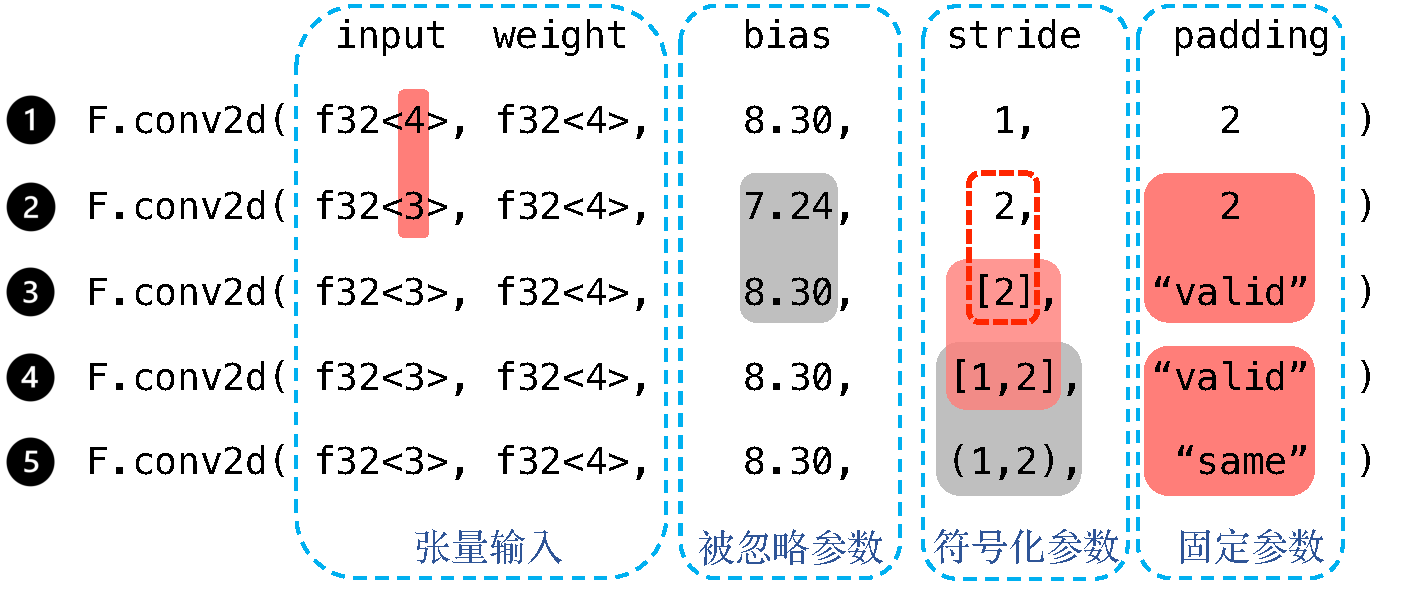
\includegraphics[width=1.\linewidth]{figures/conv2d.pdf}
    \caption{将二维卷积接口的多个具体算子分类为不同偏算子的示例}
    \label{fig:conv2d}
\end{figure}

\begin{itemize}
    \item 对于所有输入参数,其类型固定。如图 \ref{fig:conv2d} 中的第 2、3 个具体算子,它们的参数 \texttt{stride} 和 \texttt{padding} 都有着不同的类型,因此二者属于不同的偏算子。不过,对于张量、标量、字符串、可遍历容器和数据类型以外的类型,我们认为它们不会影响规则推断,如 \texttt{torch.device} ,因此予以忽略。
    \item 对于张量,其维数固定。如第 1、2 个具体算子,其第一个输入张量 \texttt{input} 的形状分别为 $(N, C, H, W)$ 与 $(C, H, W)$ ,前者维数为 4 而后者维数为 3 ,因此二者属于不同的偏算子。这是为了使张量形状符号化之后符号的个数相同。
    \item 对于字符串和布尔型,其值固定。如第 4、5 个具体算子的 \texttt{padding} 值均为字符串类型,但值不相等,因此二者属于不同的偏算子。这是由于字符串和布尔型的变化对接口行为的影响较大,如果将其符号化并加入偏算子规则的表达,往往需要规则的表达和推断算法支持分支语义,而不仅限于代数运算,难度和复杂度将上升。相比之下,对于整型、浮点型和复数则没有额外要求,如第 2、3 个具体算子的 \texttt{bias} 参数虽然不同,但不是将他们归类为两个偏算子的原因。
    \item 对于可遍历容器,首先递归地正规化为列表类型,然后对其元素进行递归处理。如第 3、4 个具体算子的 \texttt{stride} 参数均为列表,但是其长度不相同,因此二者属于不同的偏算子。第 4、5 个具体算子的 \texttt{stride} 参数类型分别为元组和列表,但是正规化为列表后,每个元素均满足上述要求,因此不是将他们归类为两个偏算子的原因。
\end{itemize}
对于满足上述规则的偏算子,其规则与约束推导相比原接口更加容易。外部合作者仅实现了支持简单语法的推导算法,就可以为大部分算子推导符号化规则与约束,并最终提高模糊测试的覆盖率。

\section{混合算子计算图生成算法}

类比混合执行结合具体执行与符号执行的思想,我们改进 NNSmith 中的计算图生成算法,设计可以同时利用 NNSmith 中的符号化算子与本文工作中的具体算子的混合算子计算图生成算法。

混合执行对符号执行的改进之处在于,不会累积符号化规则直到最后再求解,而是面对难以符号化表达的逻辑,及时进行随机具体化。类似地,我们对 NNSmith 中符号化计算图生成算法的改进之处在于,不会累积符号化规则与约束直至图中节点达到预设值才求解,而是在插入每一个算子时进行及时的随机具体化,每一步插入结束时都能得到一个具体化的计算图。

由于我们对 NNSmith 的计算图生成算法做改进,因而在此不再完整地赘述整体的计算图生成算法,而是介绍对其中前向算子插入逻辑的改动。算法 \ref{algo:hygen} 描述了向计算图 $G$ 中插入一个新算子的过程,其顶层逻辑为随机选择以下两种算子插入模式:
\begin{itemize}
    \item \textbf{插入符号化算子。}符号化算子包括两种: NNSmith 中由人工编写规则定义的符号化算子,和基于本文工作中的偏算子进行规则与约束推理得到的符号化算子。首先我们从全部符号化算子中随机选择一个算子,然后枚举计算图中所有与这个算子的输入张量组合在维数和数据类型上一致的张量组合。因为实验中我们不会生成算子个数大于 10 的计算图,因而此处枚举操作的时间开销不至于过大。接着我们考虑每一个符合要求的张量组合,将其代入选定的算子对输入张量形状的符号约束,并用 SMT 求解器进行求解。如果成功得到了一组解,则据此将选定的算子立即具体化,并插入到计算图中。对比 NNSmith ,此处没有将符号规则与约束累积到最后求解,因此每一步插入前后计算图都是具体化的。
    \item \textbf{插入具体算子。} 具体算子的插入本质上是计算图中已有张量组合与具体算子的输入张量组合之间的匹配。例如,计算图中已有两个 \texttt{float32} 类型的张量,形状分别为 \texttt{[8,4,5,5]} 和 \texttt{[4,4,3,3]} ;而具体算子 \texttt{F.conv2d} 的输入恰好也是 \texttt{float32} 类型的形状分别为 \texttt{[8,4,5,5]} 和 \texttt{[4,4,3,3]} 的张量,于是,便可以将两个已有张量分别作为具体算子 \texttt{F.conv2d} 的两个输入,从而插入一个新的具体算子。一般地,我们枚举计算图中所有的张量组合,组合的枚举可以用全局容器进行缓存优化,在每一步插入新算子后进行更新,以避免冗余计算。对于每一种已经存在的张量组合,我们在具体算子数据集中查找是否有输入张量组合恰好与之一致的算子,若有则将其插入到计算图中。为了提高查找效率,我们提前建立了张量形状与数据类型的不同组合到具体算子的映射。
\end{itemize}

\begin{algorithm}
    \caption{混合算子计算图生成算法中的前向算子插入 \texttt{ForwardInsert($\cdot$)}}
    \label{algo:hygen}
\KwIn{计算图 $G$, 符号化算子集合 $\Phi_s$, 具体算子集合 $\mathcal{C}$}
% \KwOut{具体算子集合 $C$}
\SetKw{KwIs}{is}
\SetKw{Continue}{continue}
\SetKwProg{Fn}{Function}{:}{}

\SetKwFunction{FForwardInsert}{ForwardInsert}
\SetKwFunction{FForwardInsertSymbOp}{ForwardInsertSymbOp}
\SetKwFunction{FForwardInsertConcreteOp}{ForwardInsertConcreteOp}

\Fn{\FForwardInsert{$G$}} {
    \uIf{$\texttt{uniform\_sample(0,1)} < 0.5$} {
        % $\phi_s \gets$ 随机选取一个符号化算子\;
        $\phi_s \gets$ $\Phi_s$\texttt{.sample()}\;
        \texttt{ForwardInsertSymbOp}($G$, $\phi_s$)\;
    }
    \Else{
        \texttt{ForwardInsertConcreteOp}($G$)\;
    }
}

\Fn{\FForwardInsertSymbOp{$G$, $\phi_s$}} {
    % $\mathcal{I} \gets$ $G$ 中所有维数与数据类型与 $\phi_s$ 的输入一致的张量组合
    $\mathcal{I} \gets$ $G$.\texttt{tensor\_combinations}($\phi_s$\texttt{.input.ranks}, $\phi_s$\texttt{.input.dtypes})\;
    \For{$i \in \mathcal{I}$} {
        $m \gets \phi$\texttt{.requires}($i$)\;
        $s \gets$ \texttt{solver.solve}($m$)\;
        \If{$s$} {
            $\phi_c \gets \phi$\texttt{.concretize\_by}($s$)\;
            $G$\texttt{.insert\_consumer}($i, \phi_c$)\;
        }
    }
}

\Fn{\FForwardInsertConcreteOp{$G$}} {
    \For{$t \in G$.\texttt{tensor\_combinations}} {
        $\mathcal{C}_\text{cand} \gets \mathcal{C}$\texttt{.lookup}($t$)\;
        $c \gets \mathcal{C}_\text{cand}$\texttt{.sample()}\;
        $G$\texttt{.insert\_consumer}($t, c$)\;
    }
}

\end{algorithm}

\section{差分测试与漏洞寻找}

与 NNSmith 相同,对每个从计算图生成算法构造出的测例,我们分别在不启用编译器的解释执行模式,和启用编译器的图执行模式下运行,运用差分测试比较其结果。若在任一模式下执行失败,则隐式地寻找到漏洞。若在两种模式下均成功执行,但结果的差距不在误差允许范围内,则显式地寻找到漏洞。

\iffalse
\chapter{数学符号和公式}

\section{数学符号}

中文论文的数学符号默认遵循 GB/T 3102.11—1993《物理科学和技术中使用的数学符号》
\footnote{原 GB 3102.11—1993,自 2017 年 3 月 23 日起,该标准转为推荐性标准。}。
该标准参照采纳 ISO 31-11:1992 \footnote{目前已更新为 ISO 80000-2:2019。},
但是与 \TeX{} 默认的美国数学学会(AMS)的符号习惯有所区别。
具体地来说主要有以下差异:
\begin{enumerate}
  \item 大写希腊字母默认为斜体,如
    \begin{equation*}
      \Gamma \Delta \Theta \Lambda \Xi \Pi \Sigma \Upsilon \Phi \Psi \Omega.
    \end{equation*}
    注意有限增量符号 $\increment$ 固定使用正体,模板提供了 \cs{increment} 命令。
  \item 小于等于号和大于等于号使用倾斜的字形 $\le$、$\ge$。
  \item 积分号使用正体,比如 $\int$、$\oint$。
  \item
    偏微分符号 $\partial$ 使用正体。
  \item
    省略号 \cs{dots} 按照中文的习惯固定居中,比如
    \begin{equation*}
      1, 2, \dots, n \quad 1 + 2 + \dots + n.
    \end{equation*}
  \item
    实部 $\Re$ 和虚部 $\Im$ 的字体使用罗马体。
\end{enumerate}

以上数学符号样式的差异可以在模板中统一设置。
另外国标还有一些与 AMS 不同的符号使用习惯,需要用户在写作时进行处理:
\begin{enumerate}
  \item 数学常数和特殊函数名用正体,如
    \begin{equation*}
      \uppi = 3.14\dots; \quad
      \symup{i}^2 = -1; \quad
      \symup{e} = \lim_{n \to \infty} \left( 1 + \frac{1}{n} \right)^n.
    \end{equation*}
  \item 微分号使用正体,比如 $\dif y / \dif x$。
  \item 向量、矩阵和张量用粗斜体(\cs{symbf}),如 $\symbf{x}$、$\symbf{\Sigma}$、$\symbfsf{T}$。
  \item 自然对数用 $\ln x$ 不用 $\log x$。
\end{enumerate}


英文论文的数学符号使用 \TeX{} 默认的样式。
如果有必要,也可以通过设置 \verb|math-style| 选择数学符号样式。

关于量和单位推荐使用
\href{http://mirrors.ctan.org/macros/latex/contrib/siunitx/siunitx.pdf}{\pkg{siunitx}}
宏包,
可以方便地处理希腊字母以及数字与单位之间的空白,
比如:
\SI{6.4e6}{m},
\SI{9}{\micro\meter},
\si{kg.m.s^{-1}},
\SIrange{10}{20}{\degreeCelsius}。



\section{数学公式}

数学公式可以使用 \env{equation} 和 \env{equation*} 环境。
注意数学公式的引用应前后带括号,通常使用 \cs{eqref} 命令,比如式\eqref{eq:example}。
\begin{equation}
  \frac{1}{2 \uppi \symup{i}} \int_\gamma f = \sum_{k=1}^m n(\gamma; a_k) \mathscr{R}(f; a_k).
  \label{eq:example}
\end{equation}

多行公式尽可能在“=”处对齐,推荐使用 \env{align} 环境。
\begin{align}
  a & = b + c + d + e \\
    & = f + g
\end{align}



\section{数学定理}

定理环境的格式可以使用 \pkg{amsthm} 或者 \pkg{ntheorem} 宏包配置。
用户在导言区载入这两者之一后,模板会自动配置 \env{thoerem}、\env{proof} 等环境。

\begin{theorem}[Lindeberg--Lévy 中心极限定理]
  设随机变量 $X_1, X_2, \dots, X_n$ 独立同分布, 且具有期望 $\mu$ 和有限的方差 $\sigma^2 \ne 0$,
  记 $\bar{X}_n = \frac{1}{n} \sum_{i+1}^n X_i$,则
  \begin{equation}
    \lim_{n \to \infty} P \left(\frac{\sqrt{n} \left( \bar{X}_n - \mu \right)}{\sigma} \le z \right) = \Phi(z),
  \end{equation}
  其中 $\Phi(z)$ 是标准正态分布的分布函数。
\end{theorem}
\begin{proof}
  Trivial.
\end{proof}

同时模板还提供了 \env{assumption}、\env{definition}、\env{proposition}、
\env{lemma}、\env{theorem}、\env{axiom}、\env{corollary}、\env{exercise}、
\env{example}、\env{remar}、\env{problem}、\env{conjecture} 这些相关的环境。
\fi
